\RequirePackage{fixltx2e}
\documentclass{jknotes}
\usepackage{joshkirklin}

\begin{document}

\institution{Cambridge Part III Maths}
\title{String Theory}
\lecturer{Paul Townsend}
\notetaker{Josh Kirklin}
\date{Lent 2016}

\maketitle
\suggestionsspiel
In these notes, variables with arrows above them \(\vec{x}\) are ordinary spatial vectors in the temporal gauge, whereas boldface variables \(\vb{x}\) are transverse vectors in the lightcone gauge.

\tableofcontents

\section{Introduction}
\lecture{14/01/16}
An \emph{ideal string} is one with negligible cross-sectional area and uniform mass density \(\rho\). Suppose an ideal string is placed under a tension \(T\). It is a simple exercise to deduce that the speed of propagation \(v\) of a disturbance in the displacement of the string is given by \(v = \sqrt{T/\rho}\).
\begin{figure}[H]
    \centering
    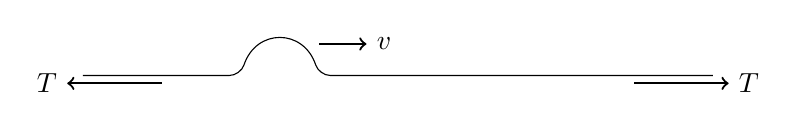
\begin{tikzpicture}
        \draw[rounded corners] (0,0) -- (2,0) .. controls (2.2,0.6) and (2.8,0.6) .. (3,0) -- (8,0);
        \draw[thick,->] (1,-0.1) -- (-0.2,-0.1) node[left] {\(T\)};
        \draw[thick,->] (7,-0.1) -- (8.2,-0.1) node[right] {\(T\)};
        \draw[thick,->] (3,0.4) -- (3.6,0.4) node[right] {\(v\)};
    \end{tikzpicture}
\end{figure}
Special relativity tells us that \(v\) must be less than or equal to \(c\) \disapprove, so we can immediately deduce the inequality \(T \le \rho c^2\). For a non-relativistic string (e.g. a violin string), \(T \ll \rho c^2\). However the strings we are interested in are said to be \emph{ultra-relativistic}: they have \(T=\rho c^2\). In this case, the only relevant quantity is \(T\).

In a quantum theory of strings, we can take advantage of Planck's constant to define a length scale for a string under tension \(T\): the \emph{string length} \(l_s \sim \sqrt{\hbar c^2/T}\). From now on, unless otherwise indicated, we will use natural units where \(\hbar=c=1\). Sometimes we will write \(T=1/2\pi\alpha'\), where \(\alpha'\) is the \emph{Regge slope parameter}, and choose \(l_s = \sqrt{\alpha'}\).

Initially, it was supposed that strings operated on an atomic scale, so that \(l_s \sim 1\) fermi \(= \SI{e-15}{\meter}\), but this failed to agree with experimental results. In electron-proton interactions, this string model predicted weak scattering, but in fact strong scattering was observed, suggesting pointlike constituent particles (eventually explained as the quarks of QCD).

A persistent prediction of all string theories is the existence of a massless spin 2 particle. This is what you would expect from a theory of quantum gravity because if you linearise general relativity about a Minkowski background you in fact obtain a massless spin 2 particle, known as the graviton.

So in 1974, string theory was reinterpreted as a theory of quantum gravity. Since we are dealing with gravity we have access to Newton's constant \(G\), and so can define another lengthscale, the Planck length \(l_P = \sqrt{\hbar G/c^3} \approx \SI{e-35}{\meter}\). Under this reinterpretation we say that the string length is on the order of magnitude of a Planck length. In fact, for string theory in a Minkowski background to be consistent, we require \(l_s\ll l_P\).

Strings can be one of two types:
\begin{figure}[H]
    \centering
    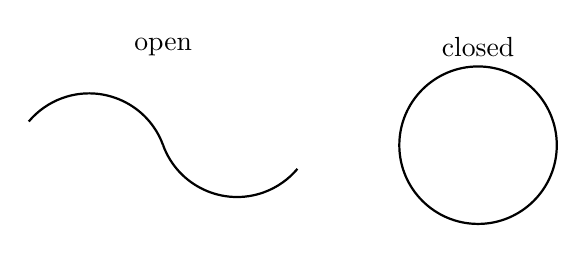
\begin{tikzpicture}[thick]
        \begin{scope}
            \node[above] at (0,1) {open};
            \draw (0,0) arc (20:140:1);
            \draw (0,0) arc (200:320:1);
        \end{scope}
        \begin{scope}
            \node[above] at (4,1) {closed};
            \draw (4,0) circle (1);
        \end{scope}
    \end{tikzpicture}
\end{figure}
As it evolves, a string sweeps out a \emph{worldsheet} in spacetime:
\begin{figure}[H]
    \centering
    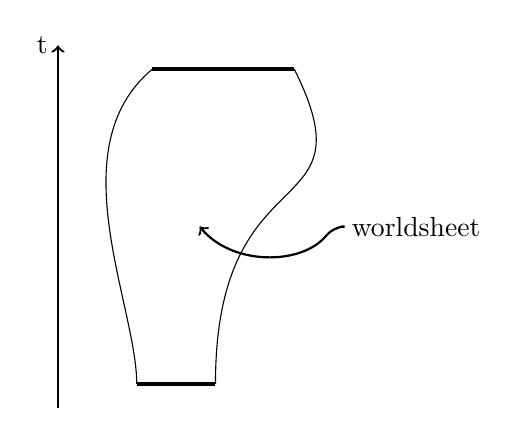
\begin{tikzpicture}
        \draw[thick,->] (0,-0.3) -- (0,4.3) node[left] {t};

        \draw[very thick] (1,0) -- (2,0);
        \draw[very thick] (1.2,4) -- (3,4);

        \draw (1,0) .. controls (1,1) and (0,3) .. (1.2,4);
        \draw (2,0) .. controls (2,3) and (4,2) .. (3,4);

        \draw[<-, thick, rounded corners] (1.8,2) .. controls (2.2,1.5) and (3.1,1.5) .. (3.5,2) -- (3.6,2) node[right] {worldsheet};
    \end{tikzpicture}
\end{figure}

They interact by splitting and joining. One of the main faults of QFT is that interactions occur at distinct points, leading to large ultraviolet divergences, but in string theory we can avoid this by imposing that the worldsheets of interacting strings must be smooth manifolds embedded in spacetime. So for example, two strings scattering off one another might be represented in the following way:
\begin{figure}[H]
    \centering
    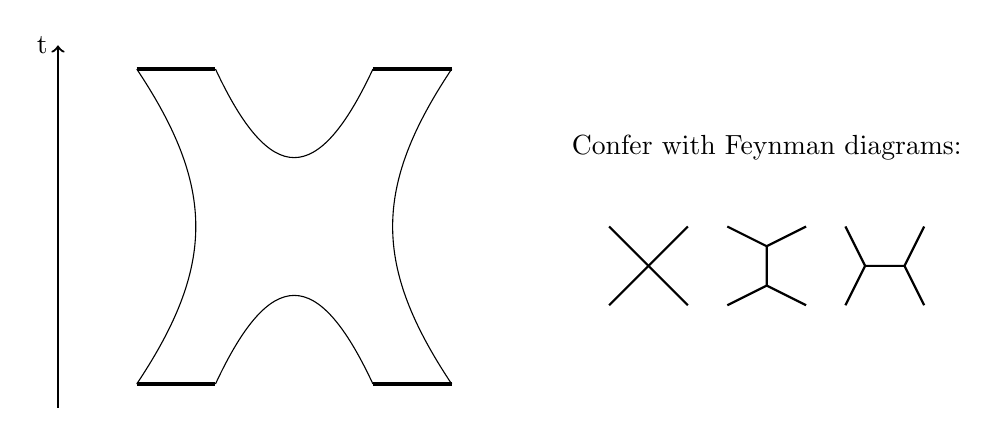
\begin{tikzpicture}
        \draw[thick,->] (0,-0.3) -- (0,4.3) node[left] {t};

        \draw[very thick] (1,0) -- (2,0);
        \draw[very thick] (4,0) -- (5,0);
        \draw[very thick] (1,4) -- (2,4);
        \draw[very thick] (4,4) -- (5,4);

        \draw (1,0) .. controls (2,1.5) and (2,2.5) .. (1,4);
        \draw (5,0) .. controls (4,1.5) and (4,2.5) .. (5,4);
        \draw (2,0) .. controls (2.7,1.5) and (3.3,1.5) .. (4,0);
        \draw (2,4) .. controls (2.7,2.5) and (3.3,2.5) .. (4,4);

        \node at (9,3) {Confer with Feynman diagrams:};

        \draw[thick](7,1) -- (8,2);
        \draw[thick](7,2) -- (8,1);

        \draw[thick](8.5,1) -- (9,1.25) -- (9,1.75) -- (8.5,2);
        \draw[thick](9.5,1) -- (9,1.25);
        \draw[thick](9.5,2) -- (9,1.75);

        \draw[thick](10,1) -- (10.25,1.5) -- (10.75,1.5) -- (11,1);
        \draw[thick](10,2) -- (10.25,1.5);
        \draw[thick](11,2) -- (10.75,1.5);
    \end{tikzpicture}
\end{figure}

Note that it is always possible to produce a closed string from an open one:
\begin{figure}[H]
    \centering
    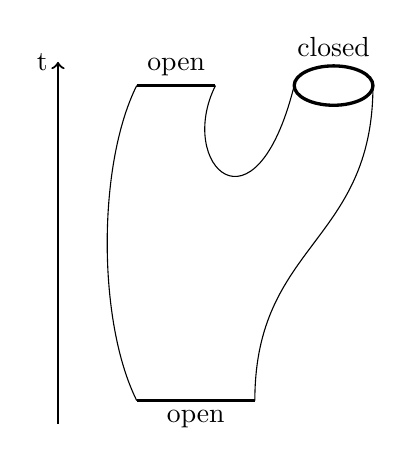
\begin{tikzpicture}
        \draw[thick,->] (0,-0.3) -- (0,4.3) node[left] {t};
        
        \draw[very thick] (1,0) -- (2.5,0);
        \draw[very thick] (1,4) -- (2,4);
        \draw[very thick] (3.5,4) ellipse (0.5 and 0.25);

        \node[below] at (1.75,0) {open};
        \node[above] at (1.5,4) {open};
        \node[above] at (3.5,4.25) {closed};

        \draw(1,0) .. controls (0.5,1) and (0.5,3) .. (1,4);
        \draw(2.5,0) .. controls (2.5,2) and (4,2) .. (4,4);
        \draw(2,4) .. controls (1.5,3) and (2.5,2) .. (3,4);
    \end{tikzpicture}
\end{figure}
Since the massless spin 2 particle appears in the spectrum of closed strings, this means that a theory of strings is always a theory of quantum gravity.

Note that strings can only interact with themselves. String theory is often popularly described as a ``Theory of Everything''. In fact, string theory must either be a ``Theory of Everything'' or a ``Theory of Nothing''. This is because if it doesn't describe everything, then certain things will not interact with gravity, but we observe that everything must interact with gravity.

There are several different types of string theory. The simplest is bosonic string theory, but it has several problems:
\begin{itemize}
    \item It allows tachyons to exist. These are particles with \(m^2 < 0\) and which lead to instabilities.
    \item As the name indicates, it does not predict fermions.
    \item Self consistency requires that \(D=26\), where \(D\) is the number of spacetime dimensions.
\end{itemize}

The only fully consistent string theories are the \emph{superstring} theories, which make use of supersymmetry. These do not allow tachyons, and have \(D=10\). In the 1980s, 5 types of superstring theory were found: Type I, Type IIA, Type IIB, Heterotic E, and Heterotic B. We will discuss Type IIA and Type IIB. All of these theories appear to be different because the coupling is weak, but in the 1990s they were unified into one (arbitrarily coupled) theory
known as \emph{M-theory}, with \(D=11\).

\section{Relativistic point particle}
\lecture{16/01/16}

What is an \emph{elementary} particle? A very mathematical definition due to Wigner is: ``a unitary irrep of the Poincar\'e group classified by mass and spin''. We however will focus on a more physical definition: ``a particle without structure''. This definition requires that the classical action of a particle depends only on the geometry of its worldline. The simplest possibility is that the action is proportional to the length of the worldline:
\begin{align}
    I &= -mc^2 \int_A^B \dd{\tau} & \text{where } & c^2\dd{\tau}^2 = -\dd{s}^2 = c^2\dd{x^0}^2 - \sum_{i=1}^{D-1}\dd{x^i}^2 \\
    \implies I &= -mc^2 \int_{t_A}^{t_B} \dd{t}\sqrt{-\dot{x}^2} && \dot{x}^m = \pdv{x^m(t)}{t},\,t = \text{arbitrary monotonic worldline time}
\end{align}
Suppose we tried to include terms involving the extrinsic curvature \(K\):
\begin{equation}
    I = -mc^2 \int_{t_A}^{t_B}\dd{t}\sqrt{-\dot{x}^2}\left( 1 + (lK)^2 + \dots \right)
\end{equation}
where \(l\) is some characteristic length scale. If \(K^{-1}\gg l\), then such extra terms are irrelevant, but this would suggest some kind of structure. So for elementary particles, we must have \(l=0\).

We have a gauge invariance in the above description: \(t\) is arbitrary. Thus we can reparametrise without consequence:
\begin{equation}
    t \rightarrow t^*(t)\quad x(t)\rightarrow x^*(t^*) = x(t)
\end{equation}
Lets check this for infinitesimal reparametrisations \(t^*(t) = t - \xi(t)\). We have:
\begin{equation}
    x^*(t-\xi(t)) = x(t) \implies \delta_\xi x(t) = x^*(t)-x(t) = \xi \dot{x}
\end{equation}
Also:
\begin{align}
    \delta_\xi \sqrt{-\dot{x}^2} &= - \frac{\dot{x}}{\sqrt{-\dot{x}^2}}\vdot\delta_\xi \dot{x} \\
    &= - \frac{\dot{x}}{\sqrt{-\dot{x}^2}}\vdot \dv{\delta_\xi x}{t} \\
    &= - \frac{\dot{x}}{\sqrt{-\dot{x}^2}}\vdot \left( \dot{\xi}\dot{x} + \xi\ddot{x} \right) \\
    &= - \dot{\xi} \sqrt{-\dot{x}^2} - \frac{\xi\dot{x}\vdot\ddot{x}}{\sqrt{-\dot{x}^2}} \\
    &= \dv{t}\left( \xi\sqrt{-\dot{x}^2} \right)
\end{align}
Therefore we have:
\begin{align}
    I(x) = -mc\int_{t_A}^{t_B} \dd{t} \sqrt{-\dot{x}^2} &\rightarrow -mc\int_{t_A^*}^{t_B^*} \dd{t^*} \sqrt{- \left( \dv{x^*}{t^*} \right)^2} \\
    &= -mc \int_{t_A-\xi(t_A)}^{t_B-\xi(t_B)} \dd{t^*} \sqrt{- \left( \dv{x^*}{t^*} \right)^2}\\
    \intertext{Relabel \(t^*\) to \(t\):}
    &= -mc \int_{t_A-\xi(t_A)}^{t_B-\xi(t_B)} \dd{t} \sqrt{-(\dot{x}^*)^2} \\
    &= -mc \int_{t_A-\xi(t_A)}^{t_B-\xi(t_B)} \dd{t} \left[ \sqrt{-\dot{x}^2} + \dv{t}\left( \xi\sqrt{-\dot{x}^2} \right) \right]
\end{align}
\begin{align}
    \implies \delta I(x) &= -mc\left( \int_{t_A-\xi(t_A)}^{t_B-\xi(t_B)} - \int_{t_A}^{t_B} \right) \dd{t} \sqrt{-\dot{x}^2} - mc \int_{t_A-\xi(t_A)}^{t_B-\xi(t_B)} \dd{t} \dv{t}\left( \xi\sqrt{-\dot{x}^2} \right) \\
    &= mc \left(\int^{t_B}_{t_B-\xi(t_B)} - \int^{t_A}_{t_A-\xi(t_A)}\right) \dd{t} \sqrt{-\dot{x}^2} -mc \left[ \xi\sqrt{-\dot{x}^2} \right]^{t_B-\xi(t_B)}_{t_A-\xi(t_A)} \\
    &= mc\left(\xi(t_B - \xi(t_B))\sqrt{-\dot{x}^2}|_{t_B-\xi(t_B)} - \xi(t_A - \xi(t_A))\sqrt{-\dot{x}^2}|_{t_A-\xi(t_A)} \right)
-mc \left[ \xi\sqrt{-\dot{x}^2} \right]^{t_B-\xi(t_B)}_{t_A-\xi(t_A)} \\
&= 0
\end{align}
as expected.

Note that gauge invariance is \emph{not} a symmetry, but instead implies redundancy. We can eliminate this by imposing a \emph{gauge condition}. For example, the \emph{temporal gauge} is \(x^0(t) = t\). In this gauge we have \(I = -mc^2\int\dd{t}\sqrt{1 - \frac{v^2}{c^2}}\) where \(v = \abs{\dv{\vec{x}}{t}}\). If we subtract the negative rest energy \(-mc^2\) and take \(c\rightarrow\infty\), we recover the normal non-relativistic action:
\begin{equation}
    I \rightarrow I_{\text{NR}} = \int\dd{t} \frac{1}{2}mv^2
\end{equation}

From now on we will take \(c = 1\).

\subsection{Hamiltonian formulation}
We have a Lagrangian \(\mathcal{L} = -m \sqrt{-\dot{x}^2}\), from which we can obtain a conjugate momentum:
\begin{equation}
    p_m = \pdv{\mathcal{L}}{\dot{x}^m} = \frac{m\dot{x}_m}{\sqrt{-\dot{x}^2}}
\end{equation}
In particular, we have \(p^2+m^2 = 0\). Not all of the components of \(p\) are independent, and we can't solve for \(\dot{x}\) in terms of \(p\). Also, the Hamiltonian is identically zero: \(H = p\vdot\dot{x}-\mathcal{L} = \frac{m\dot{x}^2}{\sqrt{-\dot{x}^2}} + m\sqrt{-\dot{x}^2} = 0\). 

Dirac's formalism (developed to deal with these cases) tells us that we should instead promote \(p\) to a free variable, and instead use a Lagrange multiplier to impose the \(p^2+m^2 = 0\) constraint. We obtain the following action:

\begin{equation}
    I[x,p;e] = \int\dd{t}\left( \dot{x}^mp_m - \frac{1}{2}e(p^2+m^2) \right)
    \tag{\(*\)}
    \label{witheinbein}
\end{equation}

\lecture{19/01/16}
We can check this is valid by eliminating \(p\) and \(e\). We have \(\fdv{I}{p}=0 \implies p = e^{-1}\dot{x}\), and we can use this to eliminate \(p\):
\begin{equation}
    I[x,p;e] \rightarrow I[x;e] = \frac{1}{2}\int\dd{t}\left( e^{-1}\dot{x}^2 - em^2 \right)
\end{equation}
We could interpret this as a sort of 1D gravity with metric \(g = -e^2\) and cosmological constant \(m^2\), coupled to \(D\) 1D scalar fields.

Now, \(\fdv{I[x;e]}{e} = 0 \implies e = \frac{\sqrt{-\dot{x}^2}}{m}\) and we can use this to eliminate \(e\):
\begin{equation}
    I[x;e] \rightarrow I[x] = -m\int\dd{t}\sqrt{-\dot{x}^2}
\end{equation}
So we regain the original action.

Note that \eqref{witheinbein} is still invariant under time reparametrisations (which we will refer to as \(\text{Diff}_1\)).

\end{document}
